\scanpage{26}
\mspage{13}
consider that \deleted{\unsure{the|that}} $\unsure{\tau|\mathcal T}$
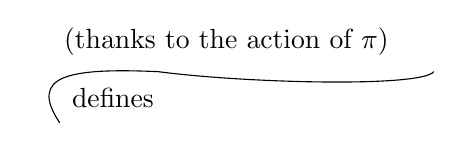
\begin{tikzpicture}[baseline=(main.base),x=1cm,y=1cm]
\node[anchor=base west,inner sep=0pt] (main) at (0,0) {defines};
\node[anchor=south west,inner sep=0pt] at (-0.10,0.65) {\inserted{(thanks to the action of $\pi$)}};
\draw[thin] (-0.15,-0.20) .. controls (-0.55,0.40) and (-0.05,0.50) .. (1.10,0.45) .. controls (2.25,0.30) and (4.45,0.25) .. (4.60,0.45);
\end{tikzpicture}
a functor
\diagram{\begin{tikzcd}[ampersand replacement=\&,row sep=large,column sep=huge]
\operatorname{Rev}(\Pi)\arrow[r,"F"]\&(\operatorname{Ens})\\
(\pi\text{-}\operatorname{Ens})\arrow[u,"
\begin{tikzpicture}[baseline=-.4ex]\node[rotate=90,inner sep=0pt] {$\approx$};\end{tikzpicture}"',"\begin{gathered}\deleted{\text{via : }\widetilde\Pi}\\E\longmapsto\widetilde\Pi^{\circ}\times_\pi E\end{gathered}"]\arrow[ur,bend right=25,"E\longmapsto\unsure{\tau|\mathcal T}^{\circ}\mathbin{\wedge}_{\pi}E"']
\end{tikzcd}}
[\uline{NB} the index $\circ$ indicates that we have reversed the actions of $\pi$, to make $\pi$ act on the right)
functor commuting with arbitrary $\varinjlim$. That said, we want $\unsure{\Gamma|F}$ (which acts on $\operatorname{Rev}(\Pi)$ via its actions on $\Pi$) to be compatible with the functor $F$, i.e. that we have isomorphisms
\[
F({}^{\gamma}\Pi')\simeq F(\Pi')
\]
$(\Pi'\in\operatorname{Ob}\operatorname{Rev}\Pi)$ functorial in $\Pi'$, and with transitivity for varying $\gamma$. We find that this means
\mspage{25}
